\documentclass[letterpaper,12pt]{article}

% Any percent sign marks a comment to the end of the line

% character encoding
\usepackage[utf8]{inputenc}
\usepackage{fontawesome}
\usepackage{tabularx}
\usepackage{ragged2e}

% Every latex document starts with a documentclass declaration like this
% The option dvips allows for graphics, 12pt is the font size, and article
%   is the style

\usepackage[pdftex]{graphicx}
\usepackage{url}
\usepackage{CJKutf8}
\usepackage[pdftex]{graphicx}


\usepackage[utf8]{inputenc}
\usepackage[TS1,T1]{fontenc}
\usepackage{fourier, heuristica}
\usepackage{array, booktabs}
\usepackage{graphicx}
\usepackage[x11names,table]{xcolor}
\usepackage{caption}
\DeclareCaptionFont{blue}{\color{LightSteelBlue3}}
\usepackage{float}
\newcommand\ytl[2]{
\parbox[b]{12em}{\hfill{\color{cyan}\bfseries\sffamily #1}~
$\cdots\cdots$~}\makebox[0pt][c]{$\bullet$}\vrule\quad 
\parbox[c]{15cm}{\vspace{7pt}\color{red!40!black!80}\raggedright\sffamily 
#2.\\[7pt]}\\[-3pt]}



% These are additional packages for "pdflatex", graphics, and to include
% hyperlinks inside a document.

\setlength{\oddsidemargin}{0.25in}
\setlength{\textwidth}{6.5in}
\setlength{\topmargin}{0in}
\setlength{\textheight}{8.5in}

% These force using more of the margins that is the default style


\title{
    \resizebox{6in}{!}{\includegraphics*{Logo}}\\
   }





\begin{document}

% Everything after this becomes content
% Replace the text between curly brackets with your own



\maketitle
% You can leave out "date" and it will be added automatically for today
% You can change the "\today" date to any text you like



\begin{center}
    \textbf{University of Viriginia, Charlottsville, VA, 22904} \\
    \rule{\textwidth}{1.2pt}
    \begin{tabular}{ c c c }
        \faGlobe https://awesome-schedule.github.io/ & \faGithub\enspace https://github.com/awesome-schedule 
    \end{tabular}
\end{center}

% This command causes the title to be created in the document

\newpage

\tableofcontents
\listoffigures
\listoftables


\newpage
\section{Executive Summary}

% An article style is separated into sections and subsections with 
%   markup such as this.  Use \section*{Principles} for unnumbered sections.

Awesome-Schedule is an open-source online scheduling website which aims to serve as 
a complement component of Student Information System (SIS) and other 
online scheduling websites, and allow students at
UVa to schedule their classes more efficiently. This is an ongoing 
project undertaken by the current undergraduate students of UVa. 
The project aims to address the issue of the current system, which is
that one online website is difficult to meet the needs of all students.
We hope to develop an adaptive website which will fit into the needs 
of the current students. In order to achieve so, we hope to 
develop this project and use it to serve as an open-source platform 
so that interested students/developers will be able to add whatever 
features they see fit. For this project, we have currently developed 
a functional scheduler, and new features are under. In the future, we hope to launch the project and 
engage an interested student community to maintain the website. 



\section{Team Profile}

\begin{description}
    \item[Zichao Hu] Chief Manager
    \item[Hanzhi Zhou] Chief Developer
    \item[Kaiying Shan] Cheif Developer
    \item[Yan Ju] Chief Marketer
\end{description}


\section{Background}
We took a survey after the beta version launch. The survey gives us many positive 
feedbacks. 
\begin{figure}
\resizebox{6in}{!}{\includegraphics*{sample_distribution}}
\caption{Participant Distribution}
\label{fig:Participant Distribution}
\end{figure}
    
\begin{figure}
\resizebox{6in}{!}{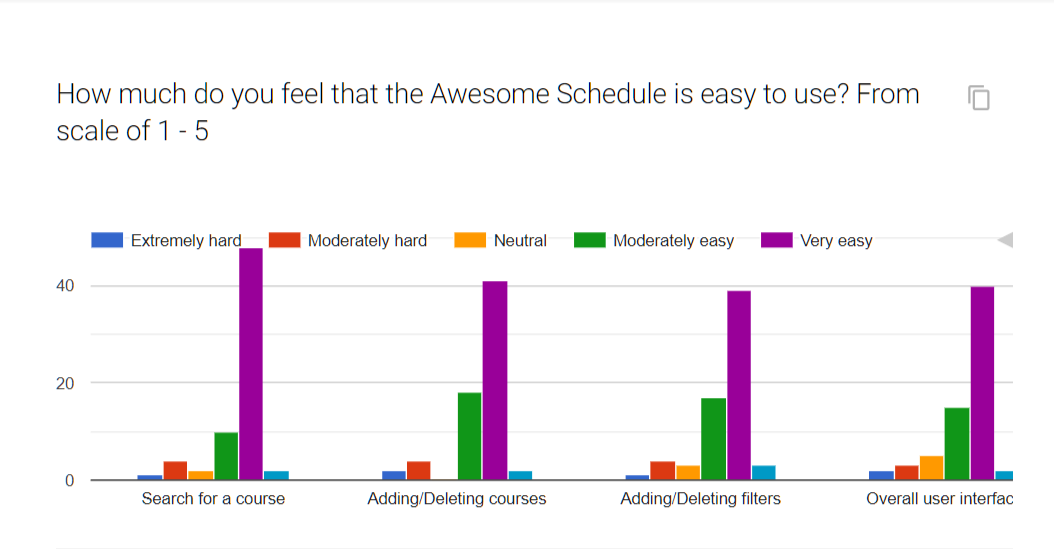
\includegraphics{UI_feedback}}
\caption{UI Feedback}
\label{fig:UI Feedback}
\end{figure}

\begin{figure}
\resizebox{6in}{!}{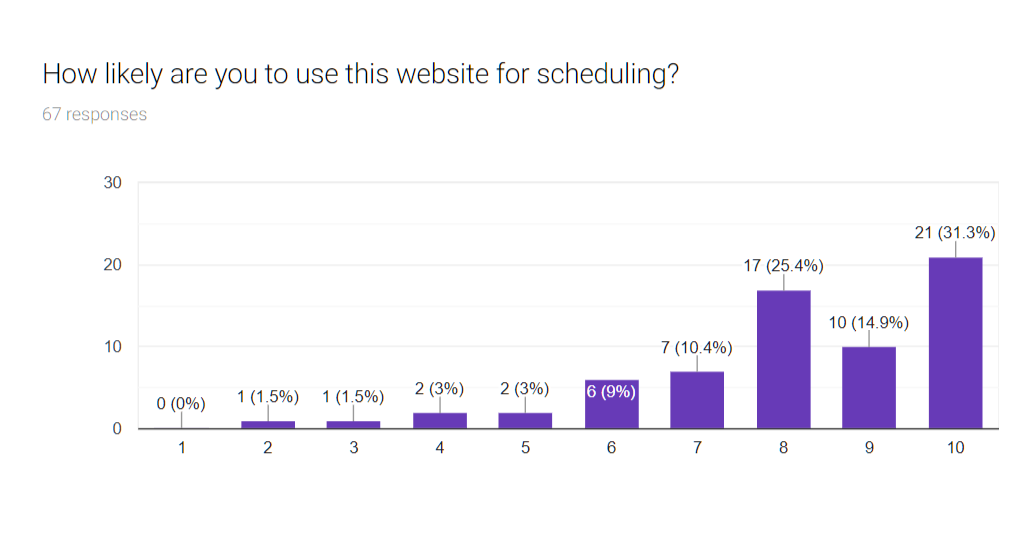
\includegraphics{potential_user}}
\caption{Potential Users}
\label{fig:Potential Users}
\end{figure}

\begin{figure}
\resizebox{6in}{!}{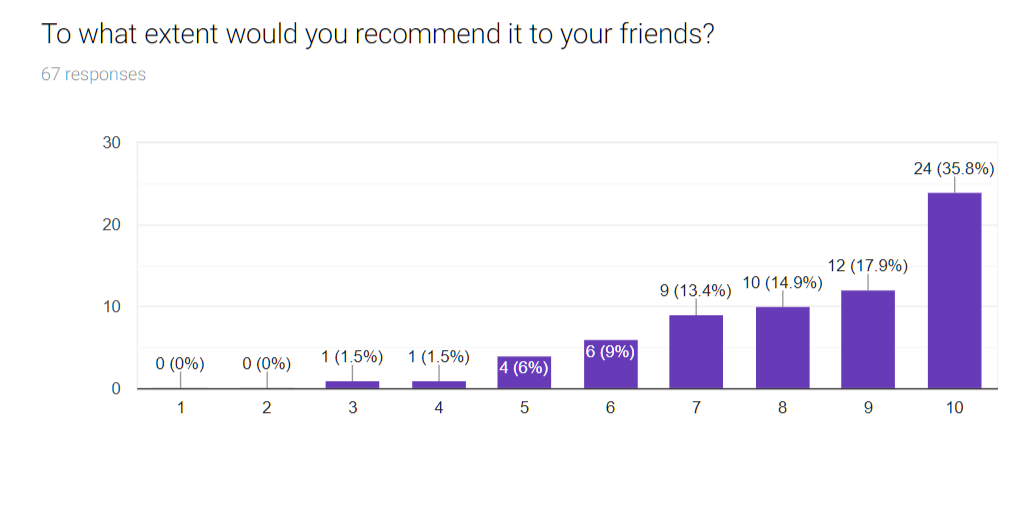
\includegraphics{potential_user2}}
\caption{Potential Users Recommendation}
\label{fig:Potential Users Recommendation}
\end{figure}


\section{TimeLine}

\begin{table}[H]
    \caption{Timeline of Awesome Schedule}
    \centering
    \begin{minipage}[t]{1.2\linewidth}
    \color{gray}
    \rule{\linewidth}{1pt}
    \ytl{03/02/2019}{Hackathon: the Beginning of the Project}
    \ytl{03/31/2019}{Beta Version Initial Launch}
    \ytl{04/05/2019}{Presentation During CS 2110 Class.\\
    Get Endorsed by Professor Basit}
    \ytl{04/09/2019}{Cooperation with CSSS}
    \ytl{04/14/2019}{Cooperation with MSN}
    \ytl{Before 05/2019}{Converstation with University Officials}
    \ytl{Before School Ends}{Recruit Potential Student Contributors}
    \ytl{05/2019}{Create Email List}
    \ytl{07/2019}{Present to the Class of 2023 Chinese Students During Sendoff}
    \ytl{08/24/2019}{Activity Fair Tabling}
    \ytl{09/2019}{Get Endorsed by Lou's List}



   
    \bigskip
    \rule{\linewidth}{1pt}%
    \end{minipage}%
    \end{table}




\section{Buget}
A preliminary budget: 
\begin{enumerate}
    \item Developing:
    \begin{itemize}
        \item Google Maps Platform: Data Request 100\$
        \item Google Analytics: Free
    \end{itemize}
    \item Marketing:
    \begin{itemize}
        \item Beta Version Launch Promotional Product: 150\$
        \item Editing Software: 60\$
        \item QRCode Generator: 60\$
        \item Flyer: 30\$
        \item Marketing Promotional Product/Poster/Tabling: 350\$
    \end{itemize}
    \item Maintenance \& Future Cost
    \begin{itemize}
        \item 150\$
    \end{itemize}
    \item  Total: 900\$

\end{enumerate}

\section{Developing Plan}
\begin{enumerate}
    \item Sticker Note Feature: \\
    \begin{itemize}
        \item Allow user to customize some time blocks 
        and insert notes to the time blocks, \textbf{e.g.} "Club meeting".
        \item User can set color for each sticker note.
        \item If serveral sticker notes have overlapping area, make each note occupy 
        part of the space and display all the notes parallel to each other, \textbf{e.g.} See Coursicle
        \item Let the users choose if each sticker note can overlap with the no-class time filter.
        \item To avoid confusion, have two separate spots for no class time and sticker notes, 
        even though sticker notes may also serve as the function of no class time, 
        \textbf{e.g.} to achive this we can add a new side bar only dedicate to the sticker note feature.
    \end{itemize}
    
    \item Comparison Feature
    \begin{itemize}
        \item Under comparison Mode, ignore the Sticker Notes Feature
        \item Compare two schedule side by side
        \item Use your imagination and creativity to make it look good and handy to use
    \end{itemize}

    \item Grade Distribution
    \begin{itemize}
        \item Create a grade distribution info for each class (not each professor
        because we do not know if the professor will still teach the class or not)
        \item Like the button of \textbf{"Click for more details (Lou's List)"}, 
        make a button next to it to show the grade distribution
        \item \textbf{Remark:} Look at the Lou's List, 
        if you click on the title of each class, e.g. CS 2110.
        There will be a pop in "Course Selection Guide". Get the data and incorporate 
        in our grade distribution
    \end{itemize}

    \item Class Distance Feature
    \begin{itemize}
        \item Create data matrix of all the buildings on Ground with their respective data
        \item Still use the "combine class" method. For each class time with
        multiple sections combined, use the section with the best distance 
        to represent those sections. Under more info, it will tell the class distance
        (in terms of time) to the previous class and the next class. 
        \item We should not calculate the class distance if the time betwen two classes are over 30 minutes.
        \item On the sidebar, we provide a new button which gives route overview of the schedule. 
        it will show the classes taken place on the google map, and the route between each class
    \end{itemize}

    \item Unit Test

    \item Export Data Feature
    \begin{itemize}
        \item Incorporate features to allow the user to add our schedule on their
        google calendar, or apple calendar
    \end{itemize}

    \item Better Mobile UI interface
    \begin{itemize}
        \item More detail discuss later
    \end{itemize}

    \item A what if scenario
    \begin{itemize}
        \item Use the data from SIS to create the what if scenario
    \end{itemize}
    
    \item "What's Cool on Ground" Feature
    \begin{itemize}
        \item add outside link to UVa CIO for advertisement. Help small but interesting CIO to get more publicity
        \item add outside link to support UVa student startup. 
        \item Provide students a new way to find interesting things going on on Ground
    \end{itemize}
\end{enumerate}

Things to heed from the results of our survey:
\begin{itemize}
    \item "accomodate to the new english program"
    \item "Make the class blocks more visually appealing, they are too plain right now" \(\times4\)
    \item "Share the class with friends" -- maybe for the comparison, we can compare with friends schedule?
    \item "The project is great. You guys are awesome"
    \item :)
\end{itemize}

\end{document}